
\chapter{Arsitektur Continer (Container Architecture)}
\authors{Richwen Canady, Desfantio Wuidjaja, Vincenzo Matalino}

\section{Latar Belakang}
Konsep container berasal dari teknologi chroot pada sistem operasi UNIX. Teknologi ini memungkinkan pengguna untuk membuat lingkungan kerja yang terisolasi pada sistem operasi UNIX. Di lingkungan kerja ini, pengguna dapat menjalankan aplikasi secara mandiri tanpa terpengaruh oleh aplikasi lain yang berjalan di sistem yang sama. Namun, teknologi chroot memiliki beberapa keterbatasan, seperti pengguna harus mengkonfigurasi secara manual, tidak mendukung manajemen sumber daya.\\
 
Pada tahun 2008, LXC (Linux Containers) mengembangkan teknologi container sebagai solusi untuk mengatasi keterbatasan teknologi chroot pada sistem operasi UNIX. Teknologi container memungkinkan pengguna untuk menjalankan aplikasi secara otomatis dan efisien dalam lingkungan terisolasi yang mudah dikelola. Teknologi kontainer berjalan di sistem operasi Linux, menggunakan kernel yang sama untuk menjalankan aplikasi di dalam container.\\

Pada 2013, Docker dirilis sebagai implementasi teknologi container yang lebih ramah pengguna dan mudah digunakan. Docker menyediakan gambar yang berisi semua elemen yang diperlukan untuk menjalankan aplikasi dalam container, termasuk aplikasi, sistem operasi, dan dependensi. Gambar Docker mudah dibuat, dikelola, dan dibagikan, dan dapat digunakan untuk penerapan cepat di lingkungan produksi.\\

Container menjadi lebih populer dan banyak digunakan untuk pengembangan dan pengelolaan aplikasi di lingkungan cloud. Container memungkinkan pengguna mengoptimalkan penggunaan sumber daya, meningkatkan portabilitas, dan mengelola aplikasi dengan mudah. Container juga mendukung orkestrasi, seperti Kubernetes, untuk mengelola aplikasi di lingkungan yang lebih kompleks. Saat ini, container adalah teknologi penting dalam pengembangan dan manajemen aplikasi.
\subsection{Virtualization vs Container Architecture}
\textit{Container architecture} dan \textit{virtualization} adalah dua teknologi yang sering digunakan dalam pengembangan dan pengelolaan aplikasi, namun ada beberapa perbedaan antara keduanya yaitu:
\begin{itemize}
	\item Isolasi= Arsitektur container menggunakan teknologi yang lebih ringan untuk menjalankan aplikasi di lingkungan yang terisolasi. Virtualisasi, di sisi lain, menggunakan teknologi hypervisor untuk mengisolasi lingkungan virtual dari sistem host. Oleh karena itu, arsitektur container lebih efisien daripada virtualisasi dalam hal penggunaan sumber daya.
	\item Sistem operasi= Arsitektur container menggunakan kernel yang sama dengan sistem operasi host untuk menjalankan aplikasi dalam container. Virtualisasi, di sisi lain, memungkinkan pengguna untuk menjalankan sistem operasi yang berbeda dalam lingkungan virtual.
	\item Portabilitas= Arsitektur container mendukung portabilitas. Pengguna dapat mengembangkan aplikasi di lingkungan pengembangan dan dengan mudah menjalankannya di lingkungan produksi. Pada saat yang sama, virtualisasi memerlukan konfigurasi yang lebih kompleks untuk menjalankan lingkungan virtual di lingkungan produksi yang berbeda.
	\item Overhead= Overhead arsitektur container lebih rendah daripada virtualisasi karena tidak memerlukan overhead hypervisor dan kernel. Oleh karena itu, arsitektur container lebih efisien dalam hal penggunaan sumber daya.
	\item Orkestrasi= Arsitektur container memungkinkan pengguna menggunakan orkestrasi (seperti Kubernetes) untuk mengelola aplikasi di lingkungan yang lebih kompleks. Virtualisasi tidak memiliki dukungan orkestrasi yang sama.
\end{itemize}

\begin{figure}[h]
	\begin{center}
	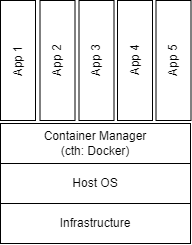
\includegraphics[width=.35\textwidth]{ContainerDiagram.png}
	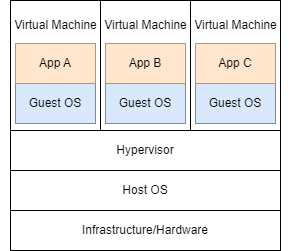
\includegraphics[width=.5\textwidth]{VirtualizationDiagram.png}
	\caption{Arsitektur Container vs Virtualization.}
	\label{fig:ContainerDiagram}
	\end{center}
\end{figure}

\section{Definisi}

\textbf{Container Architecture} merupakan sebuah konsep arsitektur yang dirancang untuk menjalankan aplikasi dalam container. Container Architecture memiliki beberapa tugas yaitu Isolasi, Portabilitas, Efisiensi, Deployment.

\textbf{Container} adalah metode menjalankan aplikasi yang memungkinkannya berjalan secara konsisten di berbagai lingkungan komputasi.\\ 
Secara sederhana, container dapat dianggap sebagai paket yang berisi semua elemen yang diperlukan untuk menjalankan aplikasi tertentu, seperti OS, library, config, dependencies, dan file penting lainnya yang dibutuhkan untuk menjalankan aplikasi tersebut.

\textbf{Docker} adalah platform open source untuk mengembangkan, menguji, dan mengimplementasikan aplikasi dalam container. 
Dalam konteks Docker, container adalah lingkungan terisolasi yang dapat berjalan di host yang sama tanpa pengaruh aplikasi atau sistem operasi lain yang berjalan di host yang sama. Container dapat dianggap sebagai paket yang berisi semua elemen yang diperlukan untuk menjalankan aplikasi tertentu, termasuk perangkat lunak, pustaka, konfigurasi, dan dependensi lainnya.

\textbf Alternatifnya {Kubernetes}, adalah platform open source untuk mengelola aplikasi dalam container yang dibuat oleh Google. Kubernetes memungkinkan pengguna untuk menjalankan, mengelola, dan mengotomatiskan penerapan aplikasi dalam container secara efisien.

\begin{figure}[h]
    \centering
    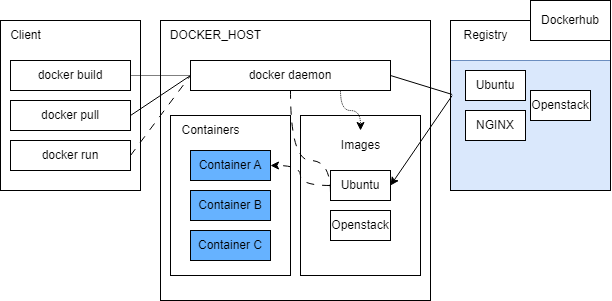
\includegraphics[width=\textwidth]{DockerDiagram.png}
    \caption{Diagram Docker.}
    \label{fig:ContainerDiagram2}
\end{figure}

\textbf{Docker image}. Image disini bukan lah Image yang kita bayangkan (.jpg, .png, etc). Image pada Docker adalah sebuah template read-only atau cuplikan/snapshot berisikan instruksi untuk membuat container yang nantinya akan dipakai. Docker Image membuat Container untuk dijalankan di Docker Platform. Analoginya, Docker image itu seperti blueprint apartemen. 

\textbf{Docker Build}. Cara membuat Docker image adalah dengan membuat file Dockerfile (yaitu instruksi pembuatan imagenya) dan menggunakan "docker build" pada dockerfile tersebut. 

\textbf{Docker Pull} adalah perintah untuk mendownload/pull image docker dari registry(cth Dockerhub)

\textbf{Docker Registry} adalah sebuah repository berbagai docker images yang dibagikan oleh para developer.

\textbf {Docker Run} adalah perintah untuk menjalankan docker images dan membentuk Docker Container berdasarkan image yang dipilih.

\textbf {Docker Container} adalah instansi Container hasil dijalankannya image yang bisa distart, stop, restart, ataupun dihapus. Analoginya, inilah ruangan Kos apartemen hasil blueprint.

\textbf {Docker Daemon} adalah mesin/engine yang berjalan di mesin host dan memanage semua proses pada docker. Semua perintah perintah diatas seperti docker run itu dikirim ke docker daemon dan dijalankan.

\section{Kelebihan dan Kekurangan}
Berikut adalah kelebihan dan kekurangan docker:


\subsection{Kelebihan}
Keuntungan dari menggunakan docker adalah:
\begin{itemize}
\item Docker mempunyai konfigurasi yang \textit{sederhana} yang dapat disesuaikan dengan kebutuhan aplikasi yang sedang dikembangkan. Dengan menetapkan beberapa baris kode yang mendukung, docker mampu membuat lingkungannya sendiri yang terpisah dari lingkungan server utama.
\item Docker memiliki tingkat keamanan yang baik. Ia akan memastikan aplikasi yang sedang berjalan tidak dapat memengaruhi container \textit{(isolation)}. Selain itu, ia juga memiliki fitur keamanan \textit{pengaturan OS host mount} dengan akses \textit{read-only} sehingga konfigurasi yang tersedia tidak akan berubah sama sekali (kecuali pengguna memiliki akses penuh).
\item Docker dapat dijalankan pada beberapa platform cloud. Karena itu, pengguna dapat melakukan porting aplikasi dengan lebih mudah dan fleksibel. Selain itu, fitur-fitur docker juga dapat dijalankan pada berbagai sistem operasi, seperti Windows, Mac, dan Linux.
\item Docker mempunyai ukuran yang cukup ringan, dan lebih hemat sumber daya. Pengguna tidak membutuhkan memory storage atau overhead yang terlalu besar untuk menggunakannya.
\item Docker memiliki fitur debugging. Waktu yang dibutuhkannya juga tergolong cepat, yakni hanya sekitar satu menit saja untuk melakukan proses debug pada Sandbox.
\end{itemize}

\subsection{Kekurangan}
Konsekuensi dari menggunakan docker adalah sebagai berikut:
\begin{itemize}
\item Walaupun dapat digunakan pada berbagai macam OS, docker mempunyai kompatibilitas \textit{cross-platform} yang kurang fleksibel. Ketika sebuah aplikasi dirancang menggunakan Windows, pengguna memerlukan bantuan \textit{tools} eksternal untuk menjalankannya di Linux.
\item Secara garis besar, docker memiliki kekurangan fitur yang harus diakali pengguna dengan cara meng-install perangkat lunak eksternal apabila pengguna tidak ingin melakukan manajemen manual. Contohnya, docker tidak mempunyai dukungan untuk health-check, atau pemrograman ulang otomatis dari node yang tidak aktif.
\end{itemize}

\section{Contoh Kasus Penggunaan Container Architecture}

Biasanya, Container Architecture ergo Docker Container dibutuhkan dalam pembuatan dan deploy aplikasi yang terdiri dari beberapa komponen berbeda, seperti {aplikasi web} yang terdiri dari server web, database, dan layanan lainnya.

Dengan menggunakan Docker, kita dapat mengemas setiap komponen aplikasi ke dalam container yang terisolasi dan dapat dijalankan secara independen di berbagai lingkungan, seperti lingkungan pengembangan, pengujian, dan produksi. Container Docker memungkinkan pengembang untuk menjamin bahwa aplikasi yang mereka kembangkan dapat dijalankan dengan konsisten di seluruh lingkungan, sehingga mengurangi risiko terjadinya kesalahan dan masalah ketika aplikasi dideploy.

Tanpa container/docker, dalam pembuatan aplikasi kita biasanya harus install dan konfigurasi setiap komponen aplikasi secara manual di setiap environment, seperti environment pengembangan, pengujian, dan produksi. Ini bisa bermasalah ketika aplikasi dideploy di lingkungan yang berbeda, karena berbeda konfigurasi dan pengaturannya. 

\textbf{Contoh kasus}, misal ada sebuah aplikasi php yang sudah didevelop menggunakan php7, belum tentu aplikasi tersebut bisa dijalankan di komputer lain yang menjalankan php5. Dengan menggunakan docker, meskipun pada dasarnya komputernya menggunakan php5, namun image dan containernya sudah ada php7 jadinya tidak perlu konfigurasi ulang.

\section{Demo Container Architecture Menggunakan Docker}
Terdapat 2 Code yang akan di demokan,yang pertama merupakan aplikasi sistem informasi untuk skripsi di php dan sebuah aplikasi to-do list dari NodeJS yang dimana keduanya akan di \textit{containerize} melalui Docker.


\begin{figure}[h!]
	\begin{center}
	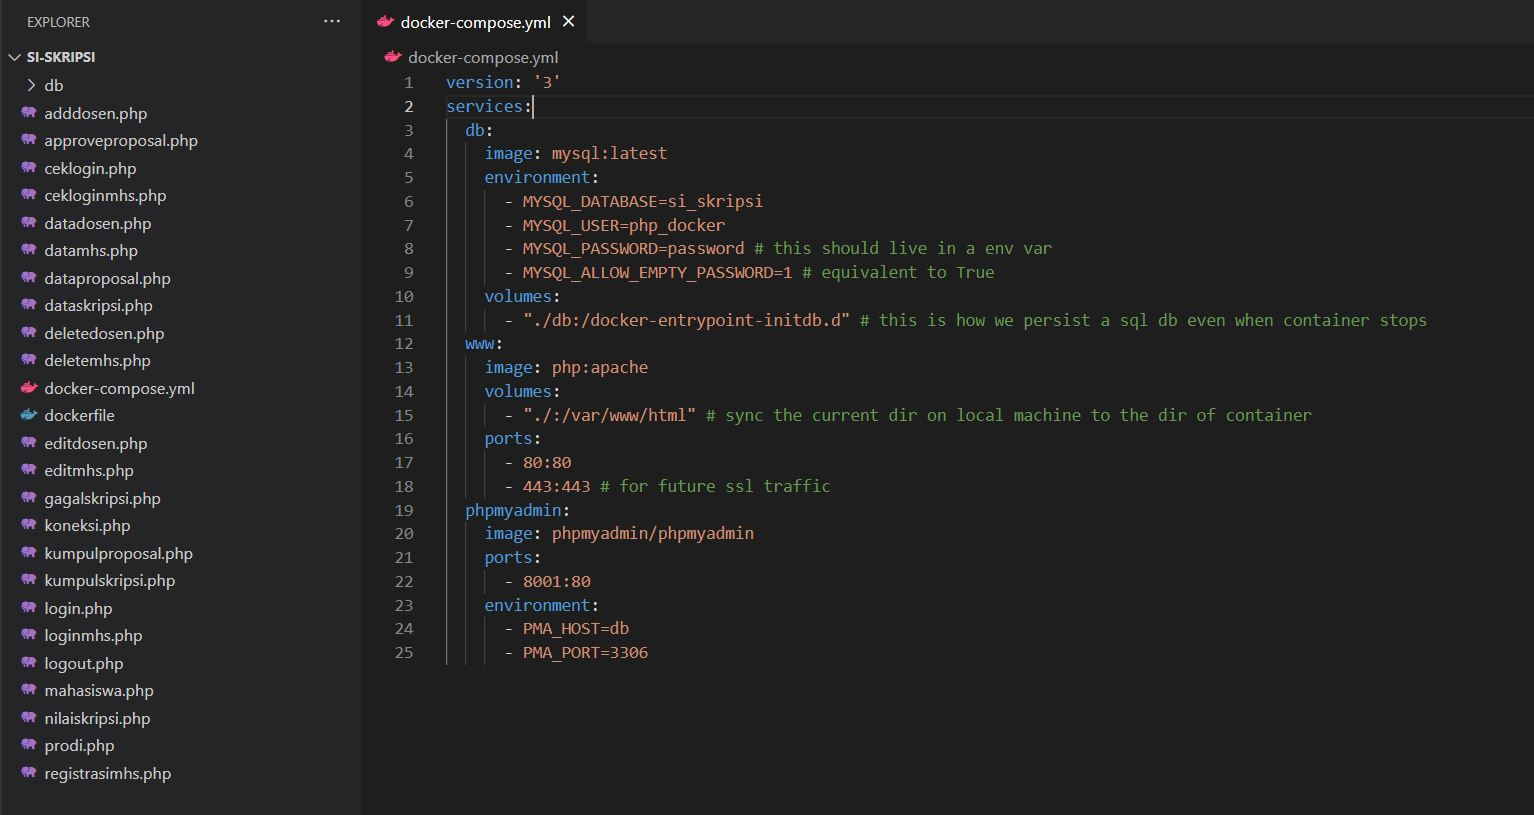
\includegraphics[width=\textwidth]{DockerDemo1.jpg}
	\caption{Aplikasi SI-Skripsi dan Docker Compose}
	\label{fig:DockerDemo1}
	\end{center}
\end{figure}

Untuk aplikasi SI-Skripsi, kami akan menggunakan Docker-Compose untuk membuat environment container yang sudah memiliki image PHP untuk bahasa pemrograman yang digunakan, Apache untuk komunikasi PHP, dan database MySQL dari docker repository. Berikut adalah code Docker-Compose.yml nya

\begin{figure}[h]
	\centering
	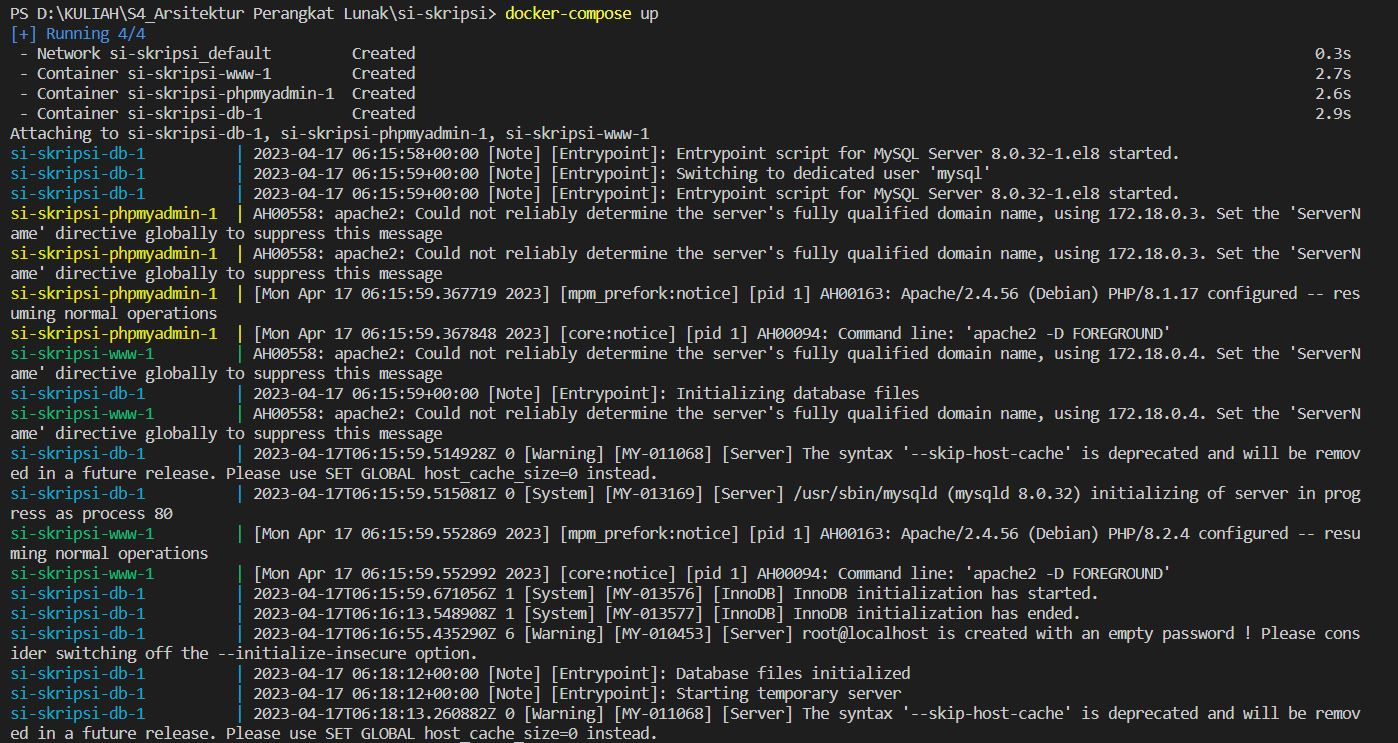
\includegraphics[width=\textwidth]{DockerDemo2.jpg}
	\caption{docker-compose up}
	\label{fig:DockerDemo2}
	
\end{figure}
Docker compose ini akan membuat 3 buah container yang akan digrup menjadi satu, yaitu container 'db' untuk MySQL, container 'www' untuk Apache, dan container phpmyadmin. Command line untuk menjalankan docker-compose.yml ini adalah docker-compose up, seperti di \textbf{Gambar 13.4}. \pagebreak

\begin{figure}[h!]
	\begin{center}
		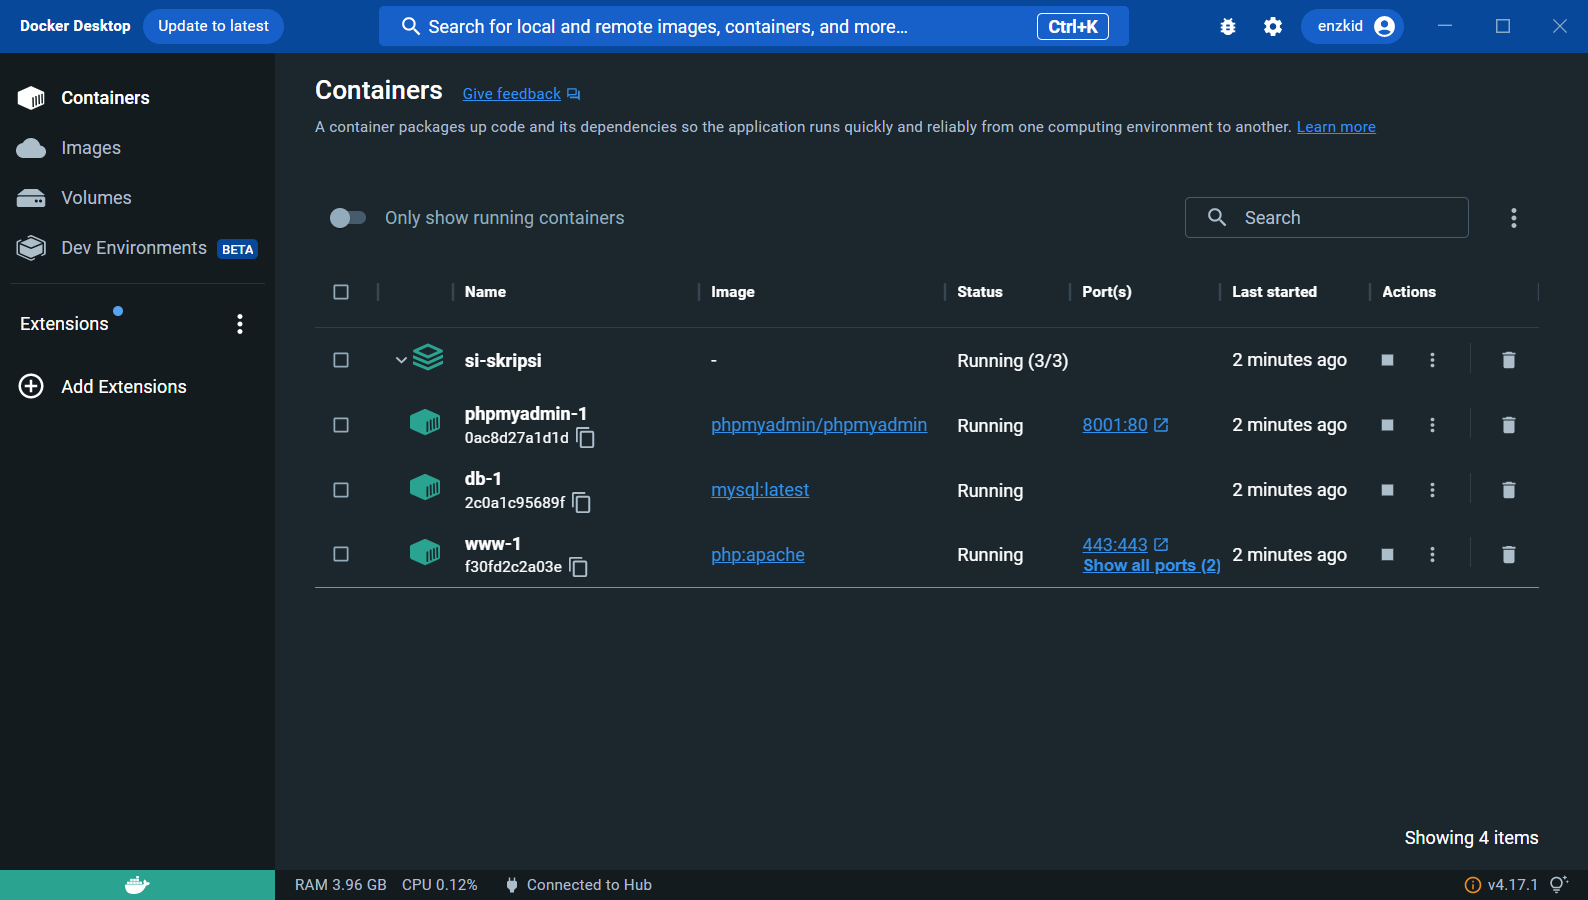
\includegraphics[width=\textwidth]{DockerDemo3.png}
		\caption{Container Docker Running}
		\label{fig:DockerDemo3}
	\end{center}
\end{figure}

\begin{figure}[h!]
	\begin{center}
		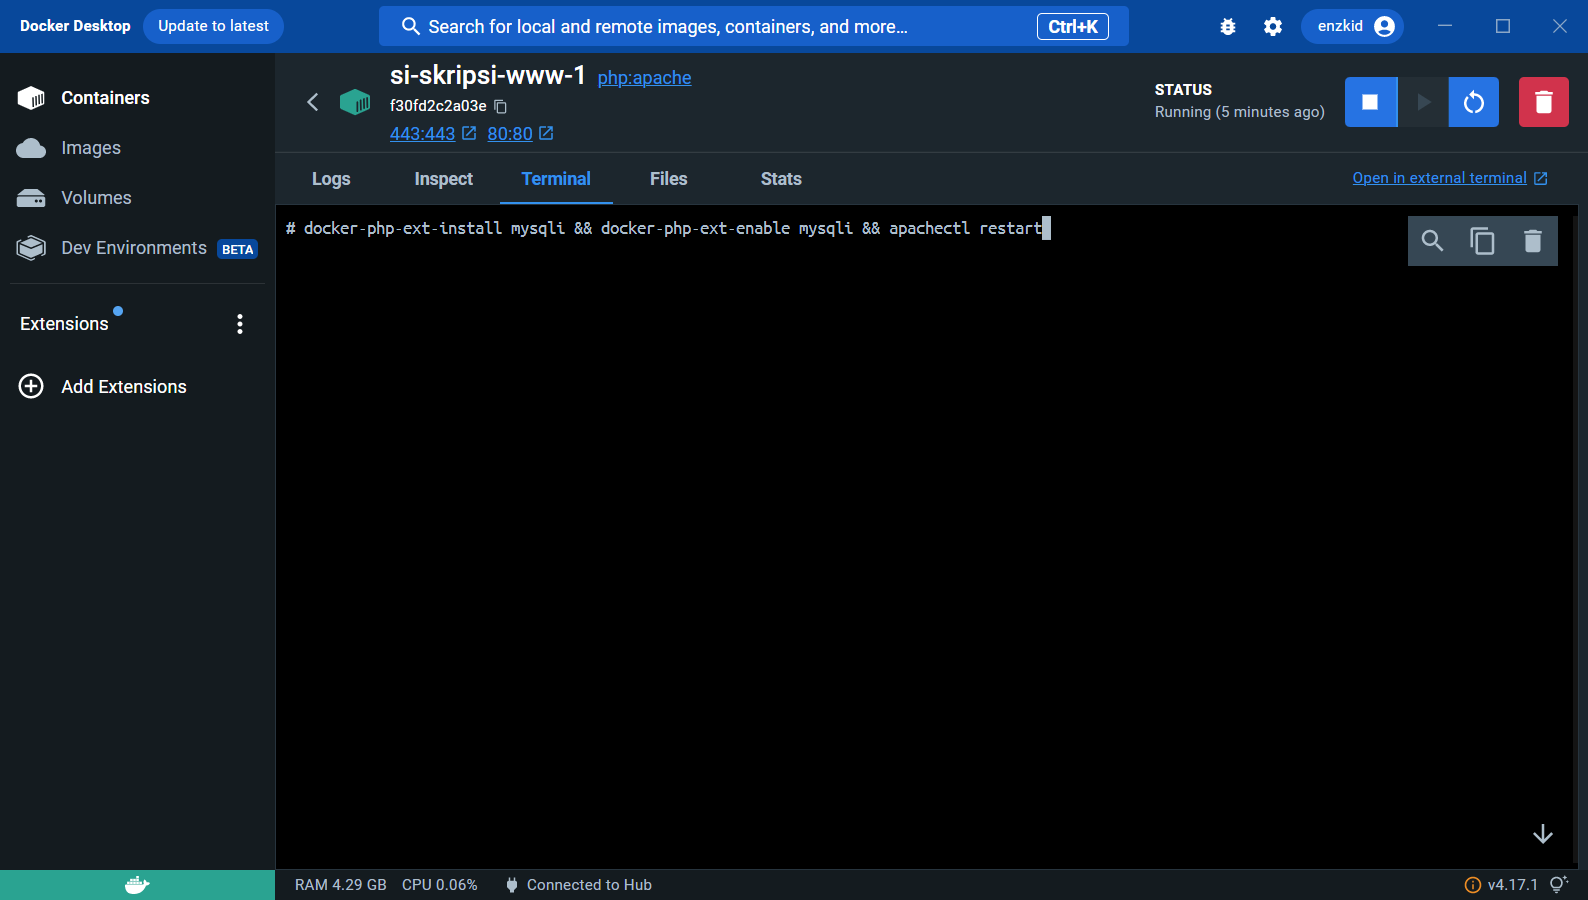
\includegraphics[width=\textwidth]{DockerDemo4.png}
		\caption{Terminal Container Apache(www)}
		\label{fig:DockerDemo4}
	\end{center}
\end{figure}

Setelah docker-compose up berhasil, container nya akan berjalan, seperti pada \textbf{Gambar 13.5}. Sebelum aplikasi bisa dijalankan perlu di \textit{install} terlebih dahulu MySQLi agar Apache bisa berkomunikasi dengan database, menggunakan line \textbf{"docker-php-ext-install mysqli \&\& docker-php-ext-enable mysqli \&\& apachectl restart"} pada terminal untuk Apache/www pada Docker, seperti pada \textbf{Gambar 13.6}.

\begin{figure}[h]
	\centering
	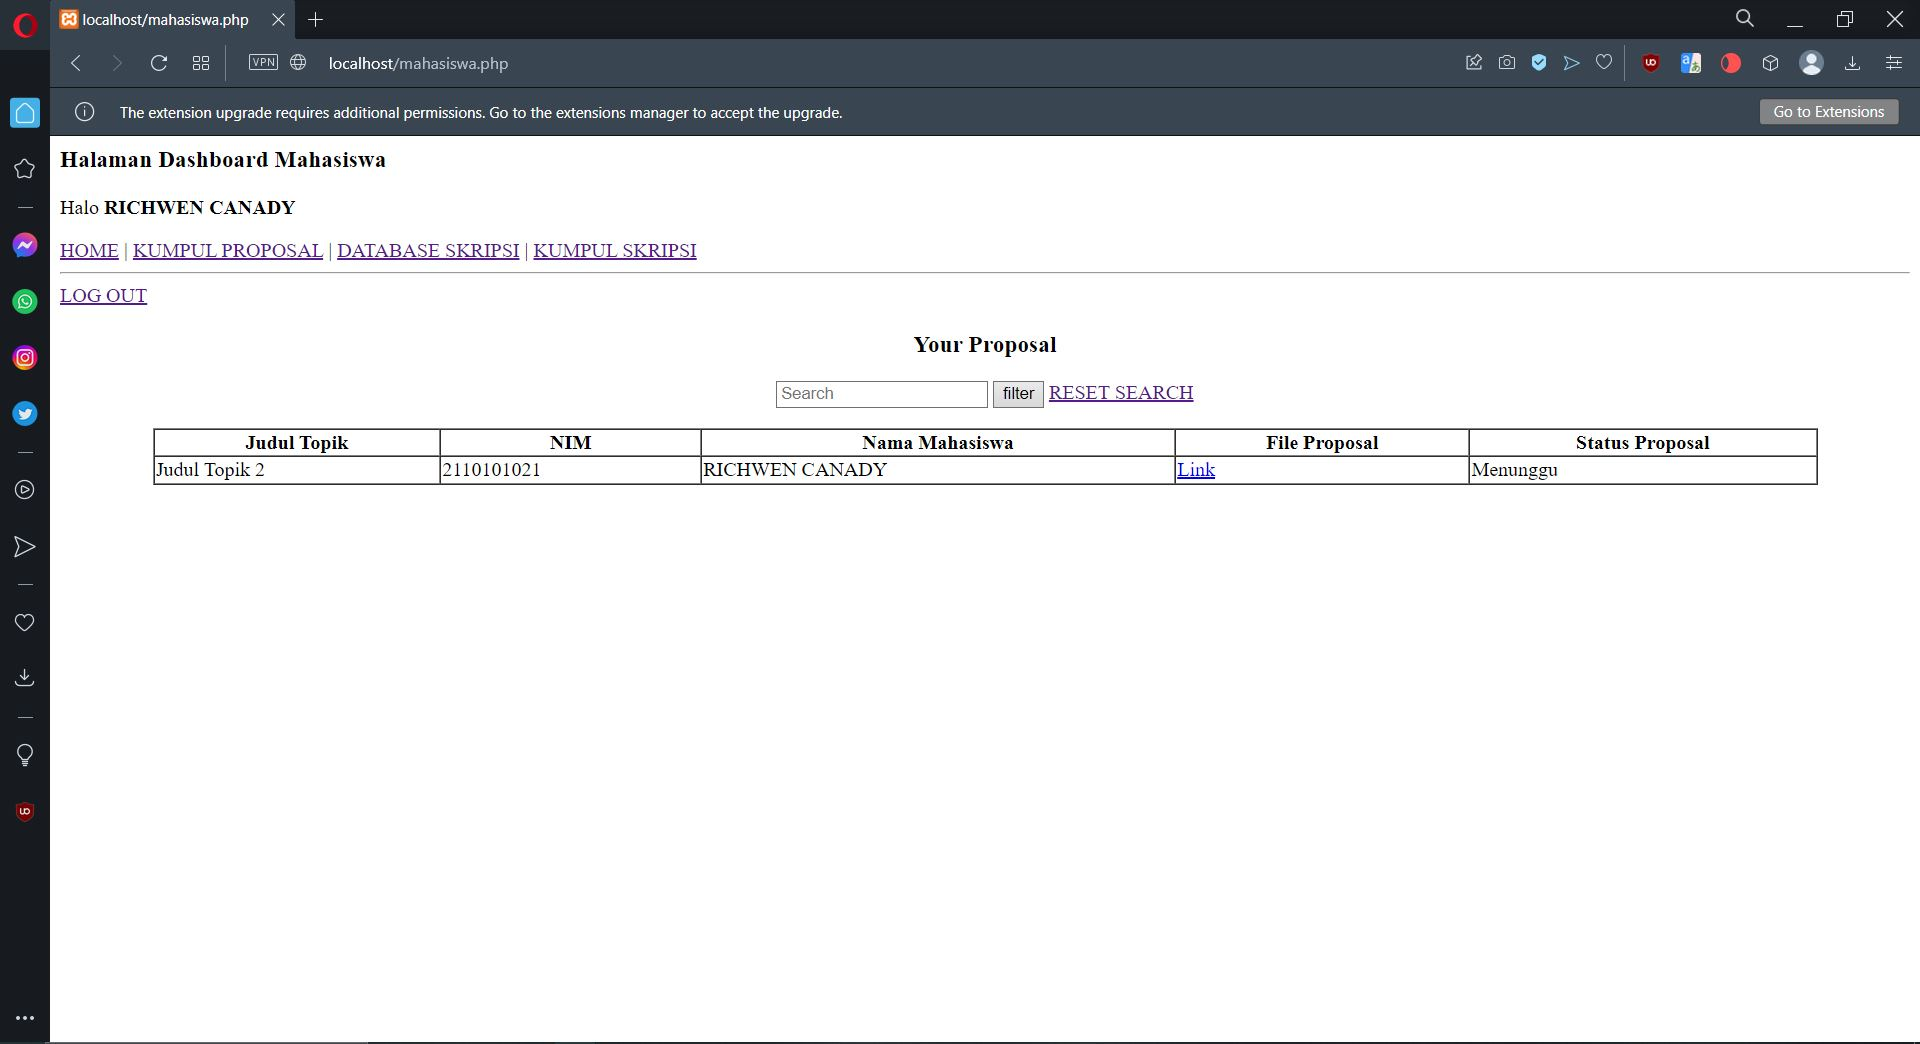
\includegraphics[width=\textwidth]{DockerDemo5.jpg}
	\caption{SI-Skripsi berjalan di Localhost}
	\label{fig:DockerDemo5}
\end{figure}

Program SI-Skripsi akan berjalan jika diakses lewat localhost seperti pada \textbf{Gambar 13.7}. Program ini berjalan di sebuah container yang terisolasi, memiliki databasenya sendiri dan tidak berpengaruh dengan xampp(Apache \& MySQL) yang dimiliki seseorang ataupun versi bahasa php seseorang. Untuk mematikan container, menggunakan command line "docker-compose down" seperti pada \textbf{Gambar 13.8}.

\begin{figure}[h]
	\centering
	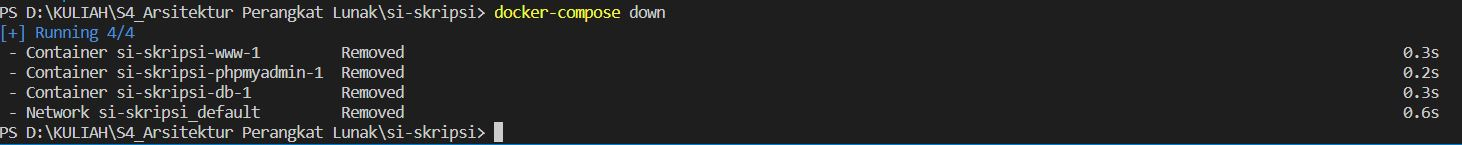
\includegraphics[width=\textwidth]{DockerDemo6.jpg}
	\caption{docker-compose down}
	\label{fig:DockerDemo6}
\end{figure}

Selanjutnya adalah aplikasi To-Do List yang dibangun dengan bahasa NodeJS, kami membuat sebuah image menggunakan file "Dockerfile". Kami akan membuat sebuah image dengan NodeJS Alpine Linux untuk version 18 dengan dependency tambahan yaitu --production menggunakan \textbf{'yarn'}, sebuah package manager mirip npm. Setelah itu kami membuild dockerfile tersebut dengan command line "\textbf{docker build -t getting-started .}" Code bisa dilihat pada \textbf{Gambar 13.9}

\begin{figure}[h]
	\centering
	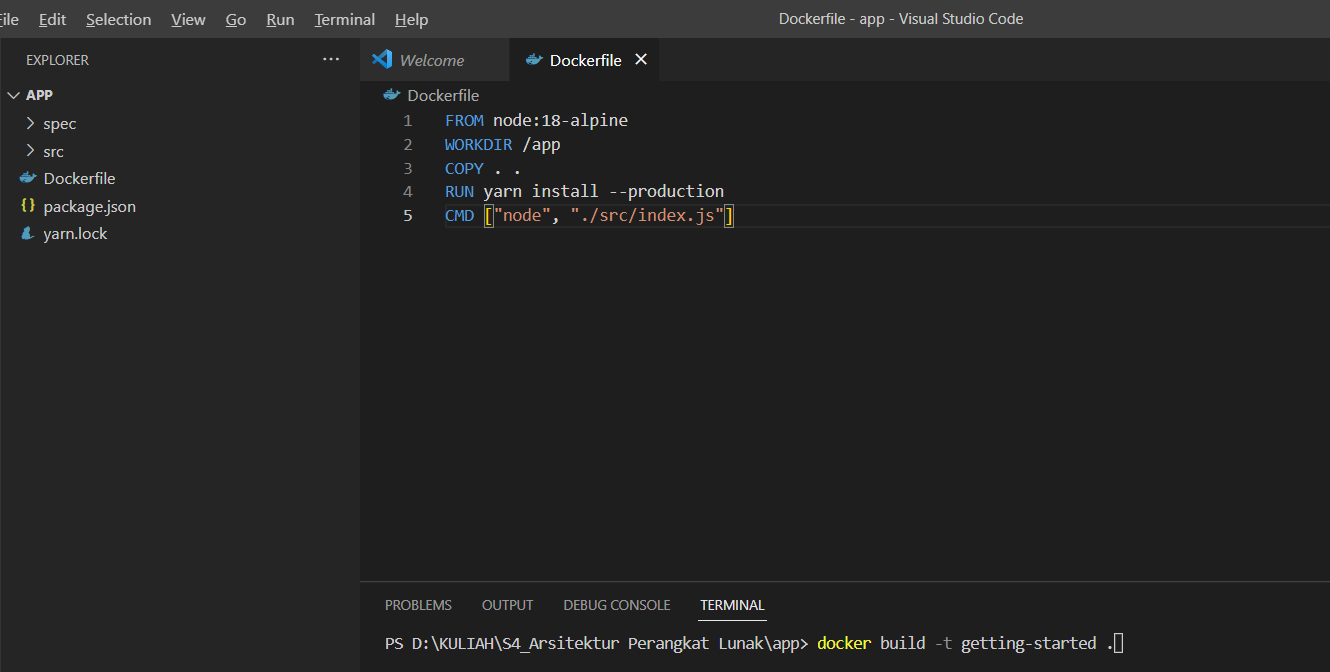
\includegraphics[width=\textwidth]{DockerDemo7.png}
	\caption{Dockerfile \& Docker Build}
	\label{fig:DockerDemo7}
\end{figure}

\begin{figure}[h!]
	\centering
	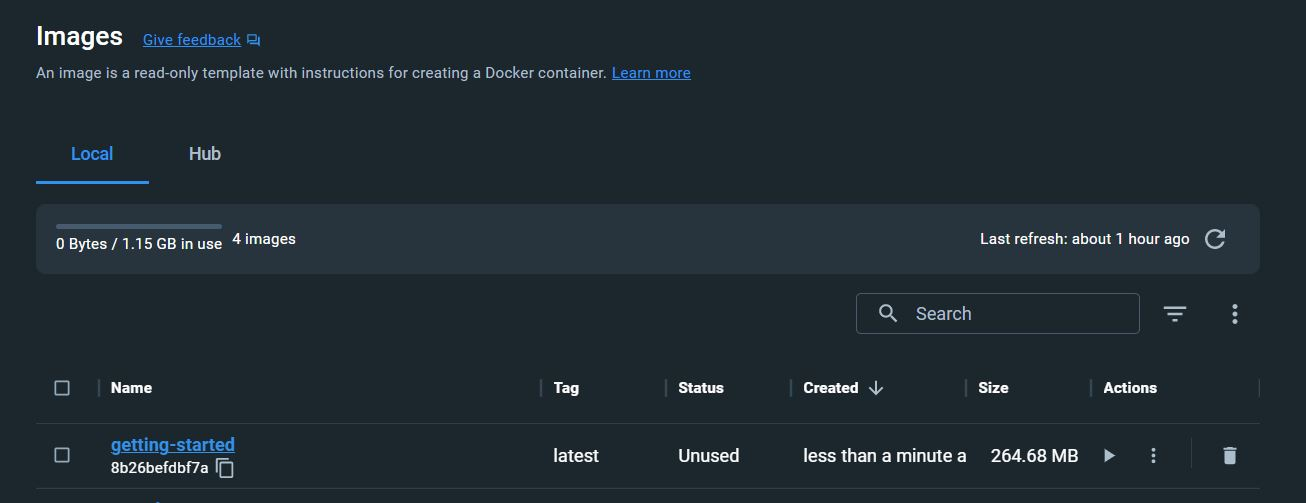
\includegraphics[width=\textwidth]{DockerDemo8.jpg}
	\caption{Image getting-started}
	\label{fig:DockerDemo8}
\end{figure}

Jika docker build telah berhasil, maka akan ada image baru yang akan muncul dengan nama "getting-started" seperti pada \textbf{Gambar 13.10}.

Kita bisa menjalankan image tersebut lewat Dockernya langsung namun untuk demo ini saya akan menggunakan command line "\textbf{docker run -dp 3000:3000 getting-started}" untuk menjalankannya di port 3000:3000.

\begin{figure}[h]
	\centering
	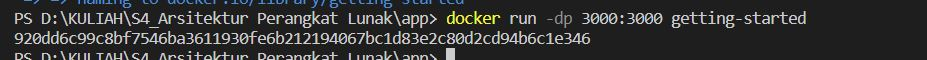
\includegraphics[width=\textwidth]{DockerDemo9.jpg}
	\caption{Docker run}
	\label{fig:DockerDemo9}
\end{figure}

Kita dapat mengecek apakah Docker Run berhasil dengan melihat apakah container kita sudah berjalan. Jika sudah berhasil akan muncul suatu container baru di port tersebut, seperti pada \textbf{Gambar 13.12}.

\begin{figure}[h]
	\centering
	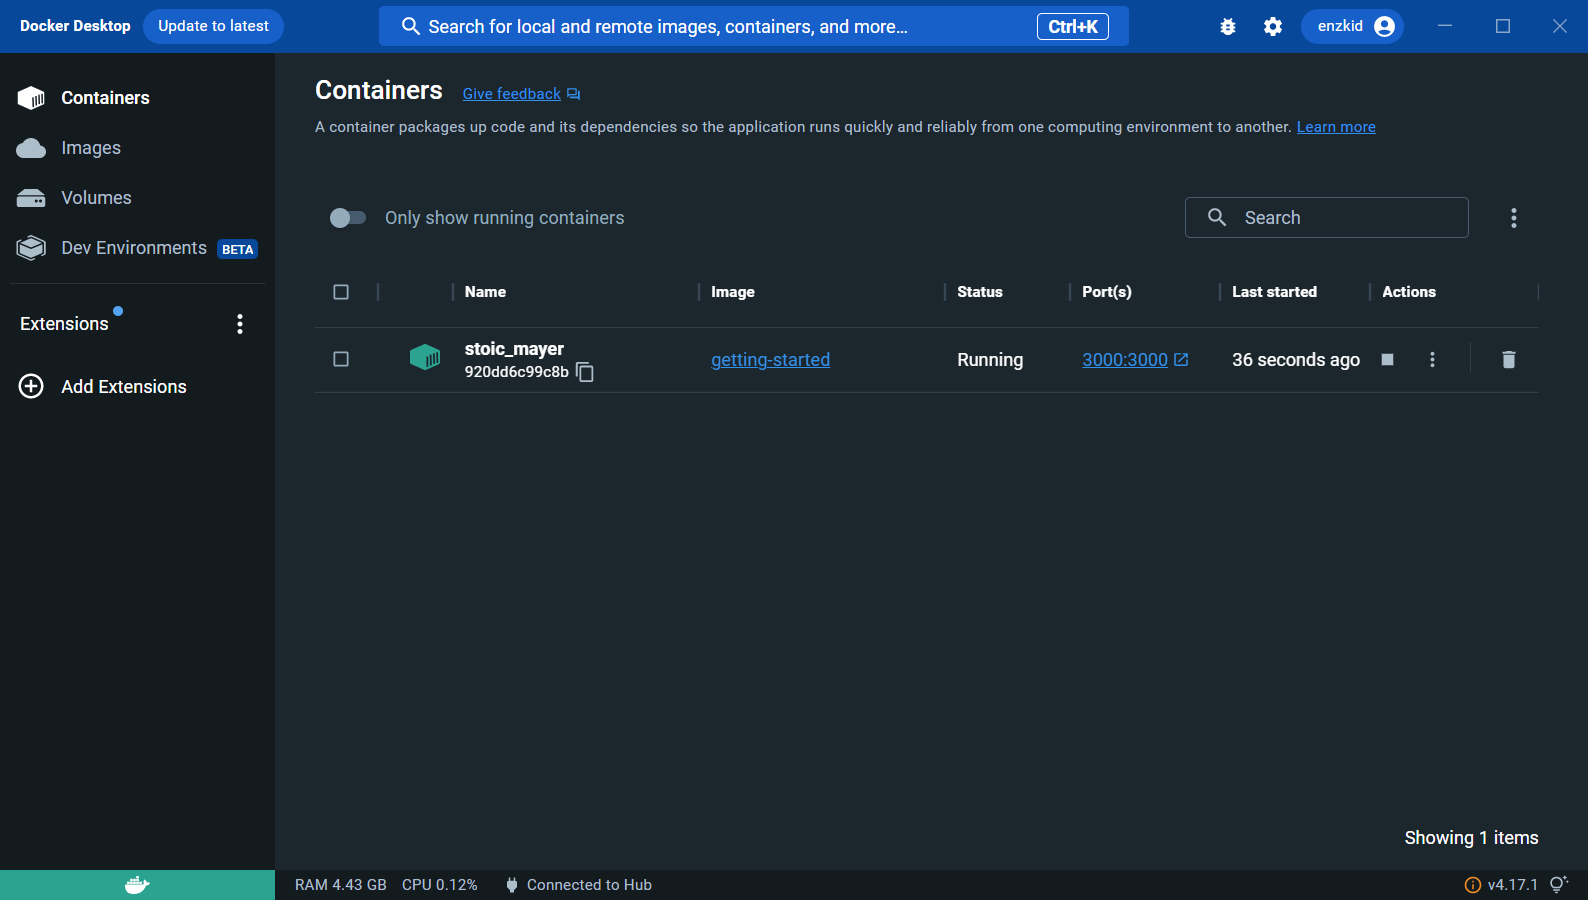
\includegraphics[width=\textwidth]{DockerDemo10.png}
	\caption{Docker Container Getting-started}
	\label{fig:DockerDemo10}
\end{figure}

\pagebreak Dan program To-do List yang dibuat dengan Node JS akan bisa diakses jika mengunjungi localhost:3000, yang dimana program ini sudah tercontainerisasi dengan versi node nya sendiri dan dependencynya sendiri.

\begin{figure}[h]
	\centering
	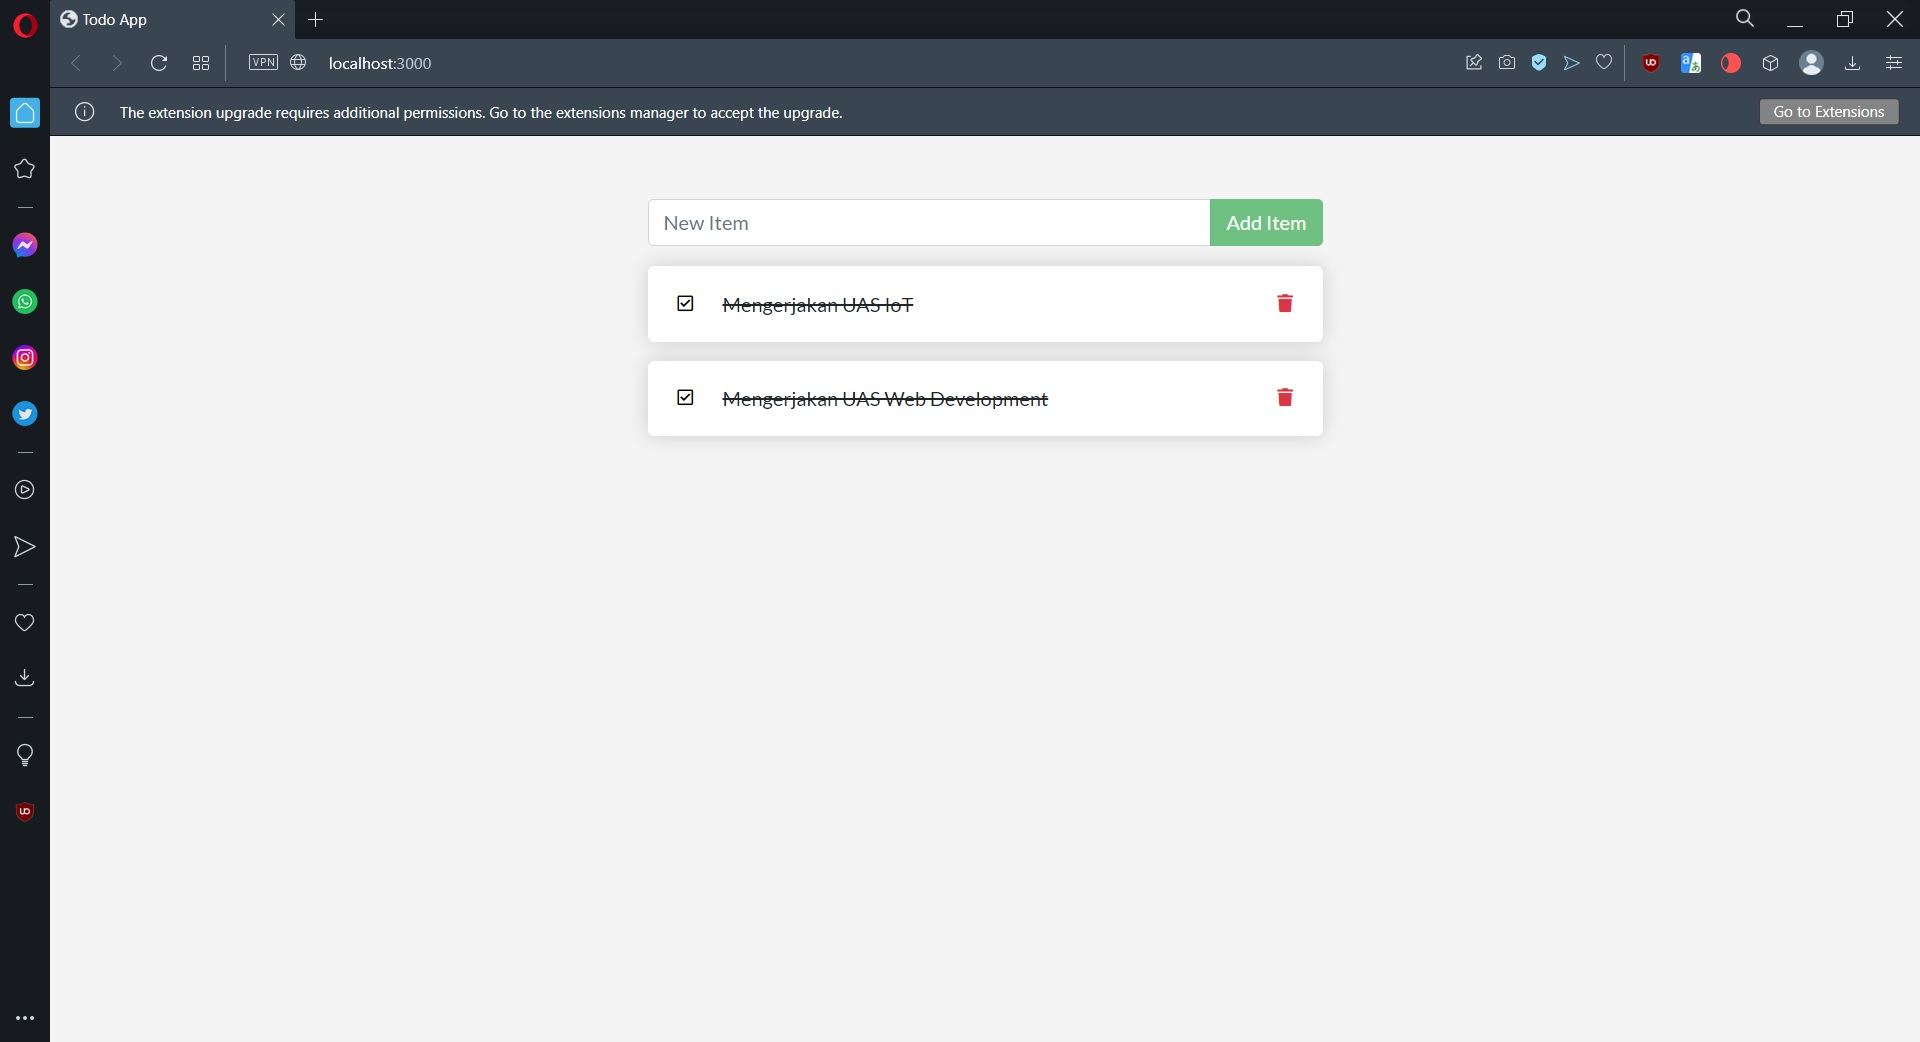
\includegraphics[width=\textwidth]{DockerDemo11.jpg}
	\caption{Aplikasi To-Do List berjalan di Container}
	\label{fig:DockerDemo11}
\end{figure}
